\langsection[subsection]{Basic Vehicle Control}{Основы управления}

\langsection[subsubsection]{Body Position}{Поза и посадка}

\begin{langblock}{0.425}
	\begin{eng}
	To control a motorcycle well:
	\begin{itemize}
		\item Posture --- Sit so you can use your arms to steer the motorcycle rather than to hold yourself up.
		\item Seat --- Sit far enough forward so that arms are slightly bent when you hold the handlegrips. Bending your arms permits you to press on the handlebars without having to stretch.
		\item Hands --- Hold the handgrips firmly to keep your grip over rough surfaces. Start with your right wrist flat. This will help you keep from accidentally using too much throttle. Also, adjust the handlebars so your hands are even with or below your elbows. This permits you to use the proper muscles for precision steering.
		\item Knees --- Keep your knees against the gas tank to help you keep your balance as the motorcycle turns.
		\item Feet --- Keep your feet firmly on the footpegs to maintain balance. Don't drag your feet. If your foot catches on something, you can be injured and it could affect your control of the motorcycle. Keep your feet near the controls so you can get to them fast if needed. Also, don't let your toes point downward they may get caught between the road and the footpegs.
	\end{itemize}
	\end{eng}
	\begin{rus}
		Для уверенного управления мотоциклом:
		\begin{itemize}
			\item Посадка "--- сидите так, чтобы использовать руки для руления, а не для удержания равновесия.
			\item Сиденье "--- сидите достаточно далеко вперед, чтобы руки были слегка согнуты при захвате руля. Согнутые руки позволяют толкать на руль без необходимости наклоняться вперед.
			\item Кисти рук "--- надежно удерживайте рукоятки для сохранения хвата на неровных поверхностях. Начальное положение правого запястья "--- горизонтальное. Это поможет избежать случайно слишком сильного открыть газа. Кроме того, отрегулируйте руль так, чтобы ваши кисти находились на уровне или ниже локтей. Это позволяет задействовать нужные мышцы для точного руления.
			\item Колени "--- прижимайте колени к топливному баку для удержания равновесия при прохождении поворотов.
			\item Ступни "--- держите ступни на подножках для удержания равновесия. Не волочите ноги по дороге. Если ваша нога за что-то зацепится, вы можете получить травму или потерять управление мотоциклом. Держите ступни возле органов управления, чтобы быстро воспользоваться ими при необходимости. Также не опускайте носки вниз "--- они могут попасть между дорогой и подножками.
		\end{itemize}
\end{rus}
\end{langblock}




\begin{figure}[htbp]
	\centering
	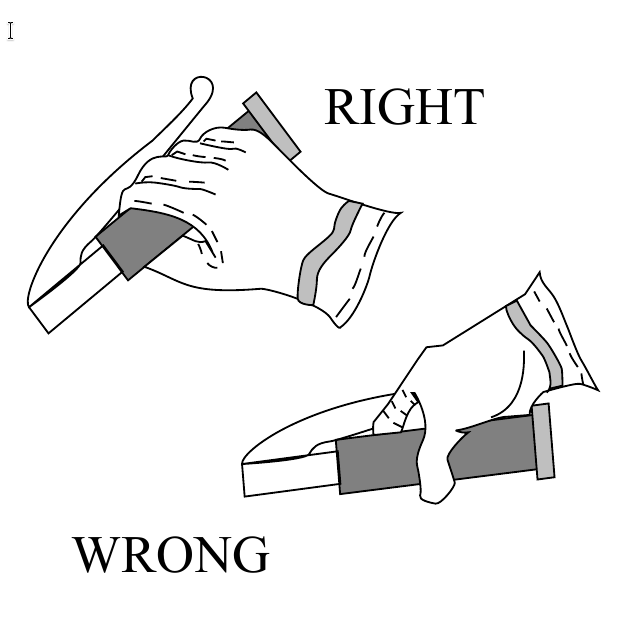
\includegraphics[width=0.45\textwidth, frame]{hold_hand_grip}
	\caption{Holding hand grips}
	\label{fig:holding_hand_grips}
\end{figure}






\langsection[subsubsection]{Shifting Gears}{Переключение передач}

\begin{langblock}{0.425}
	\begin{eng}
	There is more to shifting gears than simply getting the motorcycle to pick up speed smoothly. Learning to use the gears when downshifting, turning, or starting on hills is important for safe motorcycle operation.
	
	Shift down through the gears with the clutch as you slow or stop. Remain in first gear while you are stopped so that you can move out quickly if you need to.
	
	Make certain you are riding slowly enough when you shift into a lower gear. If not, the motorcycle will lurch, and the rear wheel may skid. When riding downhill or shifting into first gear you may need to use the brakes to slow enough before downshifting safely. Work towards a smooth, even clutch release, especially when downshifting.
	
	It is best to change gears before entering a turn. However, sometimes shifting while in the turn is necessary. If so, remember to do so smoothly. A sudden change in power to the rear wheel can cause a skid.
	\end{eng}
	\begin{rus}
		Переключение передач "--- это не просто плавный разгон мотоцикла. Умение использовать передачи для замедления, в поворотах или при старте в гору имеет важное значение для безопасной эксплуатации мотоцикла.
		
		Переключайтесь на пониженную передачу при замедлении или торможении с использованием сцепления. Перейдите на первую передачу ко времени полной остановки, чтобы иметь возможность быстро тронуться при необходимости.
		
		Убедитесь, что вы едете на приемлемой скорости перед переключением на пониженную передачу. В противном случае мотоцикл может уйдет в занос. При движении с горы или при переключении на первую передачу может потребоваться использование тормозов для снижения скорости до безопасного уровня перед понижением передачи. Стремитесь к плавному и равномерному отпусканию сцепления, особенно при переключении на пониженную передачу.
		
		Старайтесь переключиться на нужную передачу до входа в поворот. Однако иногда необходимо переключиться уже в повороте, в таком случае  делайте это очень плавно. Резкое изменение мощности на заднем колесе может вызвать занос.
\end{rus}
\end{langblock}











\langsection[subsubsection]{Braking}{Торможение}

\begin{langblock}{0.425}
	\begin{eng}
	Your motorcycle has two brakes: one each for the front and rear wheel. Use both of them at the same time. The front brake is more powerful and can provide \textbf{at least three-quarters} of your total stopping power. The front brake is safe to use if you use it properly.
	
	Remember:
	\begin{itemize}
		\item Use both brakes every time you slow or stop. Using both brakes for even ``normal`` stops will permit you to develop the proper habit or skill of using both brakes properly in an emergency. Squeeze the front brake and press down on the rear. Grabbing at the front brake or jamming down on the rear can cause the brakes to lock, resulting in control problems.
		\item If you know the technique, using both brakes in a turn is possible, although it should be done very carefully. When leaning the motorcycle some of the traction is used for cornering. Less traction is available for stopping. A skid can occur if you apply too much brake. Also, using the front brake incorrectly on a slippery surface may be hazardous. Use caution and squeeze the brake lever, never grab.
		\item Some motorcycles have integrated braking systems that link the front and rear brakes together by applying the rear brake pedal.
	\end{itemize}
	\end{eng}
	\begin{rus}
		Мотоцикл оснащен двумя независимыми тормозами: передним и задним. Используйте оба одновременно. Передний тормоз обладает большей эффективностью и может обеспечивать \textbf{не менее трех четвертей} общего тормозного усилия. Передний тормоз безопасен в использовании если делать это правильно.
		
		Помните:
		\begin{itemize}
			\item Используйте оба тормоза каждый раз при замедлении или остановке. Использование обоих тормозов даже при «обычных» остановках позволит вам выработать правильную привычку и навык их применения в экстренных ситуациях. Плавно сжимайте передний тормоз и давите на задний. Резкий захват переднего тормоза или удар по заднему может привести к блокировке колес и потере управления.
			\item Если вы владеете соответствующей техникой, можете использовать оба тормоза в повороте, однако это следует делать с особой осторожностью. При наклоне мотоцикла часть сцепления шин с дорогой расходуется для удержания в повороте. Запас сцепления для торможения остается не так много. Занос может возникнуть даже при небольшом тормозном усилии. Кроме того, неправильное использование переднего тормоза на скользком покрытии может быть опасным. Соблюдайте осторожность и плавно нажимайте рычаг тормоза, не хватайте его.
			\item Некоторые мотоциклы оснащены интегрированными тормозными системами: при нажатии на педаль заднего тормоза срабатывают оба "--- передний и задний тормоза.
		\end{itemize}
\end{rus}
\end{langblock}







\langsection[subsubsection]{Turning}{Повороты}

\begin{figure}[htbp]
	\begin{subfigure}{0.45\textwidth}
		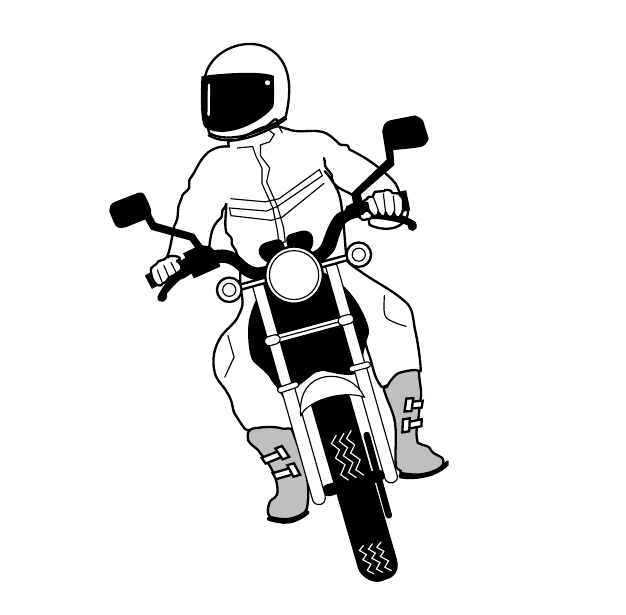
\includegraphics[width=0.95\textwidth, frame]{normal_turn}
		\caption{Normal turning}
		\label{fig:normal_turning}
	\end{subfigure}
	\hspace*{\fill}
	\begin{subfigure}{0.45\textwidth}
		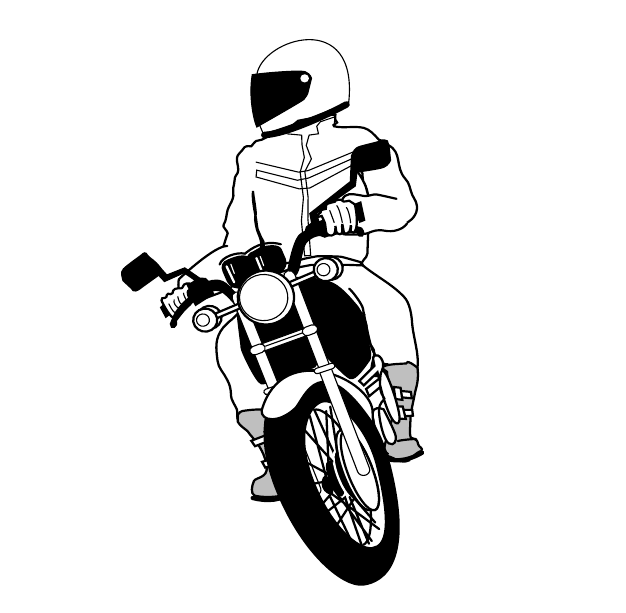
\includegraphics[width=0.95\textwidth, frame]{slow_turn}
		\caption{Slow turning}
		\label{fig:slow_turning}
	\end{subfigure}
	\caption{Turning}
	\label{fig:turning}
\end{figure}


\begin{langblock}{0.425}
	\begin{eng}
	Riders often try to take curves or turns too fast. When they can't hold the turn, they end up crossing into another lane of traffic or going off the road. Or, they overreact and brake too hard, causing a skid and loss of control. Approach turns and curves with caution.
	\begin{itemize}
		\item \textbf{SLOW} --- Reduce speed before the turn by closing the throttle and, if necessary, applying both brakes.
		\item \textbf{LOOK} --- Look through the turn to where you want to go. Turn just your head, not your shoulders, and keep your eyes level with the horizon.
		\item \textbf{PRESS} --- To turn, the motorcycle must lean. To lean the motorcycle, press on the handgrip in the direction of the turn. Press left hand-grip lean left go left. Press right handgrip lean right go right. The higher the speed in a turn the greater the lean angle.
		\item \textbf{ROLL} --- Roll on the throttle to maintain or slightly increase speed. This helps stabilize the motorcycle.
	\end{itemize}
	
	In normal turns, the rider and the motorcycle should lean together at the same angle (Fig. \ref{fig:normal_turning}). 
	In slow, tight turns, counterbalance by leaning the motorcycle only and keeping your body straight (Fig. \ref{fig:slow_turning}).
	\end{eng}
	\begin{rus}
		Водители часто пытаются проходить повороты и виражи на слишком высокой скорости. Когда они не могут удержать траекторию, они выезжают в другую полосу или съезжают с дороги. Либо они реагируют чрезмерно и слишком резко тормозят, что вызывает занос и потерю управления. К поворотам и виражам следует приближаться с осторожностью.
		\begin{itemize}
			\item \textbf{Замедление} "--- снизьте скорость до поворота, закрыв дроссельную заслонку и при необходимости применив оба тормоза.
			\item \textbf{Взгляд} "--- смотрите сквозь поворот, туда куда хотите двигаться, на выход из поворота. Поворачивайте только голову, но не плечи. Держите голову прямо, не наклоняйте ее вместе с мотоциклом (ось взгляда на уровне горизонта).
			\item \textbf{Наклон} "--- для прохождения поворота мотоцикл должен наклониться. Чтобы наклонить мотоцикл, толкните рукоятку со стороны поворота. Толкнете левую рукоятку -- мотоцикл наклонит влево -- движение пойдет влево. Толкнете правую рукоятку "--- наклон вправо "--- движение вправо. Чем выше скорость в повороте, тем больше угол наклона\footnote{Это называется <<контрруление>>, работает от 10mph и абсолютно не похоже на велосипед. Технически, просто чтобы запомнить: нажатие, наклон и направление поворота всегда совпадают}.
			\item \textbf{Газ} "--- плавно открывайте дроссельную заслонку для поддержания или небольшого увеличения скорости. Это способствует стабилизации мотоцикла.
		\end{itemize}
		В обычных поворотах вы и мотоцикл наклоняются вместе под одинаковым углом (Рис. \ref{fig:normal_turning}). 
		
		В медленных крутых поворотах используйте контр балансировку "--- наклоняйте только мотоцикл, удерживая тело прямо  (Рис. \ref{fig:slow_turning}).
\end{rus}
\end{langblock}



